\documentclass{alex_hü}

\name{Alexander Helbok}
\course{PS Physik}
\hwnumber{11}


\begin{document}
\renewcommand{\labelenumi}{(\alph{enumi})}


\begin{mybox}{1. LC-Schaltkreis mit/ohne Wechselstrom}
	\centering \( \)
	\tcblower
	\begin{enumerate}
		\item \(  \)
		\begin{flalign*}
			\tfrac{q(t)}{C} &= L \dv[2]{q}{t} &&\\
			q(t) &= q_0\cos(\tfrac{1}{\sqrt{LC}}t) &&	
		\end{flalign*}
		\begin{tikzpicture}
			\begin{axis}[
				width=350pt,
				height=250pt,
				axis lines=center,
				%y axis line style={thick},
				tick align=outside,
				xmin=0,xmax=2.4*pi,ymin=-1.1,ymax=1.5,
				xlabel style={below},
				ylabel style={left},
				xtick={pi/2, pi, 3/2*pi , 2*pi}, ytick = {-1, 1},
				xticklabels={$\frac{\pi}{2}$, $\pi$, $\frac{3\pi}{2}$, $2\pi$},
				xlabel=\small$t/\sqrt{LC}$, ylabel=$q/q_0$,
				grid=major,
				grid style={thin,densely dotted,black!20},
				%legend columns=2,
				legend style={at={(axis description cs:0.2,0.2)},anchor=east}]
				\addplot[domain=0:2.4*pi, samples=200, blue, thick] {sin(deg(x))};
				\addplot[domain=0:2.4*pi, samples=200, orange, thick] {cos(deg(x))};
   				 \draw[dashed,olive,<->] (axis cs: 0,1.05) -- node[above,text=black,font=\footnotesize]{$\phi =  \tfrac{\pi}{2}$}(axis cs: 0.5*pi,1.05);
				\legend{$q(t)$~~~,$I(t)$};
			\end{axis}
		\end{tikzpicture}\\
	\tcbline
		\item \(  \)
%		\begin{flalign*}
%			
%		\end{flalign*}
	\end{enumerate}
\end{mybox}

\begin{mybox}{2. Serienschwingkreis}
	\centering \( L = 0.1 \unit{H};\quad R = 100 \unit{\ohm};\quad C = 0.47 \unit{\micro F};\quad U_0 = 3 \unit{V} \)
	\tcblower
	\begin{enumerate}
		\item \(  \)
%		\begin{flalign*}
	%
%		\end{flalign*}
	\tcbline
		\item \(  \)
%		\begin{flalign*}
	%			
%		\end{flalign*}
	\tcbline
		\item \(  \)
%		\begin{flalign*}
	%			
%		\end{flalign*}
	\end{enumerate}
\end{mybox}

\begin{mybox}{3. Elektrische Verschiebung}
	\centering \( \)
	\tcblower
	\begin{enumerate}
		\item \(  \)
%		\begin{flalign*}
	%
%		\end{flalign*}
	\tcbline
		\item \(  \)
%		\begin{flalign*}
	%			
%		\end{flalign*}
	\tcbline
		\item \(  \)
%		\begin{flalign*}
	%			
%		\end{flalign*}
	\tcbline
		\item \(  \)
%		\begin{flalign*}
	%			
%		\end{flalign*}
	\tcbline
		\item \(  \)
%		\begin{flalign*}
	%			
%		\end{flalign*}
	\tcbline
		\item \(  \)
%		\begin{flalign*}
	%			
%		\end{flalign*}
	\end{enumerate}
\end{mybox}



\end{document}